\chapter{Experiments}
\label{ch:experiments}

\section{Datasets}
\label{sec:ds}

In this section we consider datasets that are separated in two opposing communities. The information about the opinions of each member of this community is known. Thus, we can assign internal opinions -1 and 1 to the nodes depending on their community membership\cite{tsapMatakosTerzi}.  We consider the following.

\begin{enumerate}

  \item The Karate dataset, that represents the friendships between the members of a karate club at a US university. This network is split in two equal size polarized communities around two rival karate instructors.
  
  \item The Books dataset, that is a network of US politics books. These books were published near the 2004 presidential election and sold by Amazon. These Books are classified as "Liberal", "Conservative", or "Neutral".  There are in total 43 liberal books, 49 conservative and 13 neutral.
  
  \item The Blogs dataset, a network of hyperlinks between online blogs on US politics. Blogs are classified as either Liberal or Conservative.
  
  \item The Elections dataset, this dataset is the network between the Twitter followers of Hillary Clinton and Donald Trump collected in the period 15/12/2016-15/01/2017 – around the time of the 2016 presidential elections. Members of this network are assigned an internal opinion of 1 or -1 based on which one of the two candidates they follow. We took a subsampled portion that has be done by Matakos, et al \cite{tsapMatakosTerzi}.
    
  \item The beefban dataset, a  hashtag that Twitter users used in March 2015 to signal that their posts referred to a decision by the Indian government about the consumption of beef meat in India.
  
  \item The GermanWings dataset, a  hashtag that Twitter users used after the crash of GermanWings Flight 9525.
  
\end{enumerate}


\section{Dataset statistics}
\label{sec:stats}

\begin{table}[H]
 \centering
 \caption{Stats}
 \label{tab:statistics}
 \begin{tabular}{| l || l | l | l | l |}
 \hline
  Name & \# of Nodes & \# of Edges & Avg. Degree & $\pi(z)$\\
  \hline
  \hline
  Karate & $34$ & $78$ & 4.5882 &  0.33964\\
  \hline
    books & $105$ & $441$ & 8.4 &  0.43429\\
  \hline
    beefban & $799$ & $6026$ & 15.0839 &  0.30326\\
  \hline
  polblogs & $1490$ & $16718$ & 22.4403 &  0.30983\\
  \hline
  GermanWings & $2111$ & $7329$ & 6.9436 &  0.44479\\
  \hline
  ClintonTrump & $2832$ & $18551$ & 13.1010 &  0.07582\\
  \hline
 \end{tabular}
 \end{table}
 
\vspace{20pt}
\clearpage

\section{Experiments}
\label{sec:experim}

All experiments were made with an 2,7 GHz Dual-Core Intel Core i5 on the PyCharm IDE. We can only experiment with the $Karate$ and the $Books$ dataset on all the heuristics. The $Greedy$ algorithm cannot run on the rest of the datasets because they contain thousands of nodes. The $Greedy$ algorithm needs to consider changes in the network structure so it is impossible to compute the polarization so many times.
\\
\\ 
The $FirstTopGreedy$ and the $Expressed Opinion$ can run in all datasets and us with a fairly good decrease in polarization compared to the batch algorithms. This decrease can be greater if we consider edge additions that are proportional to the size of the dataset. Greater number of edges would make $FirstTopGreedy$ nonrunnable. The $Expressed Opinion$ can run in our larger datasets with big number of additions.
\\
\\
In addition to the heuristics we use two random algorithms. The $Random$, that chooses random edges from all possible combinations and the $RandomDifferent$. The second one chooses random edges between different $z$ opinions. More specific edges that the multiplication of their expressed opinions is negative ($z_u*z_v < 0$). 
\clearpage

\begin{figure}[!htbp]
	\begin{center}
	\advance\leftskip-1.3cm
	\captionsetup{justification=centering,margin=2cm}
	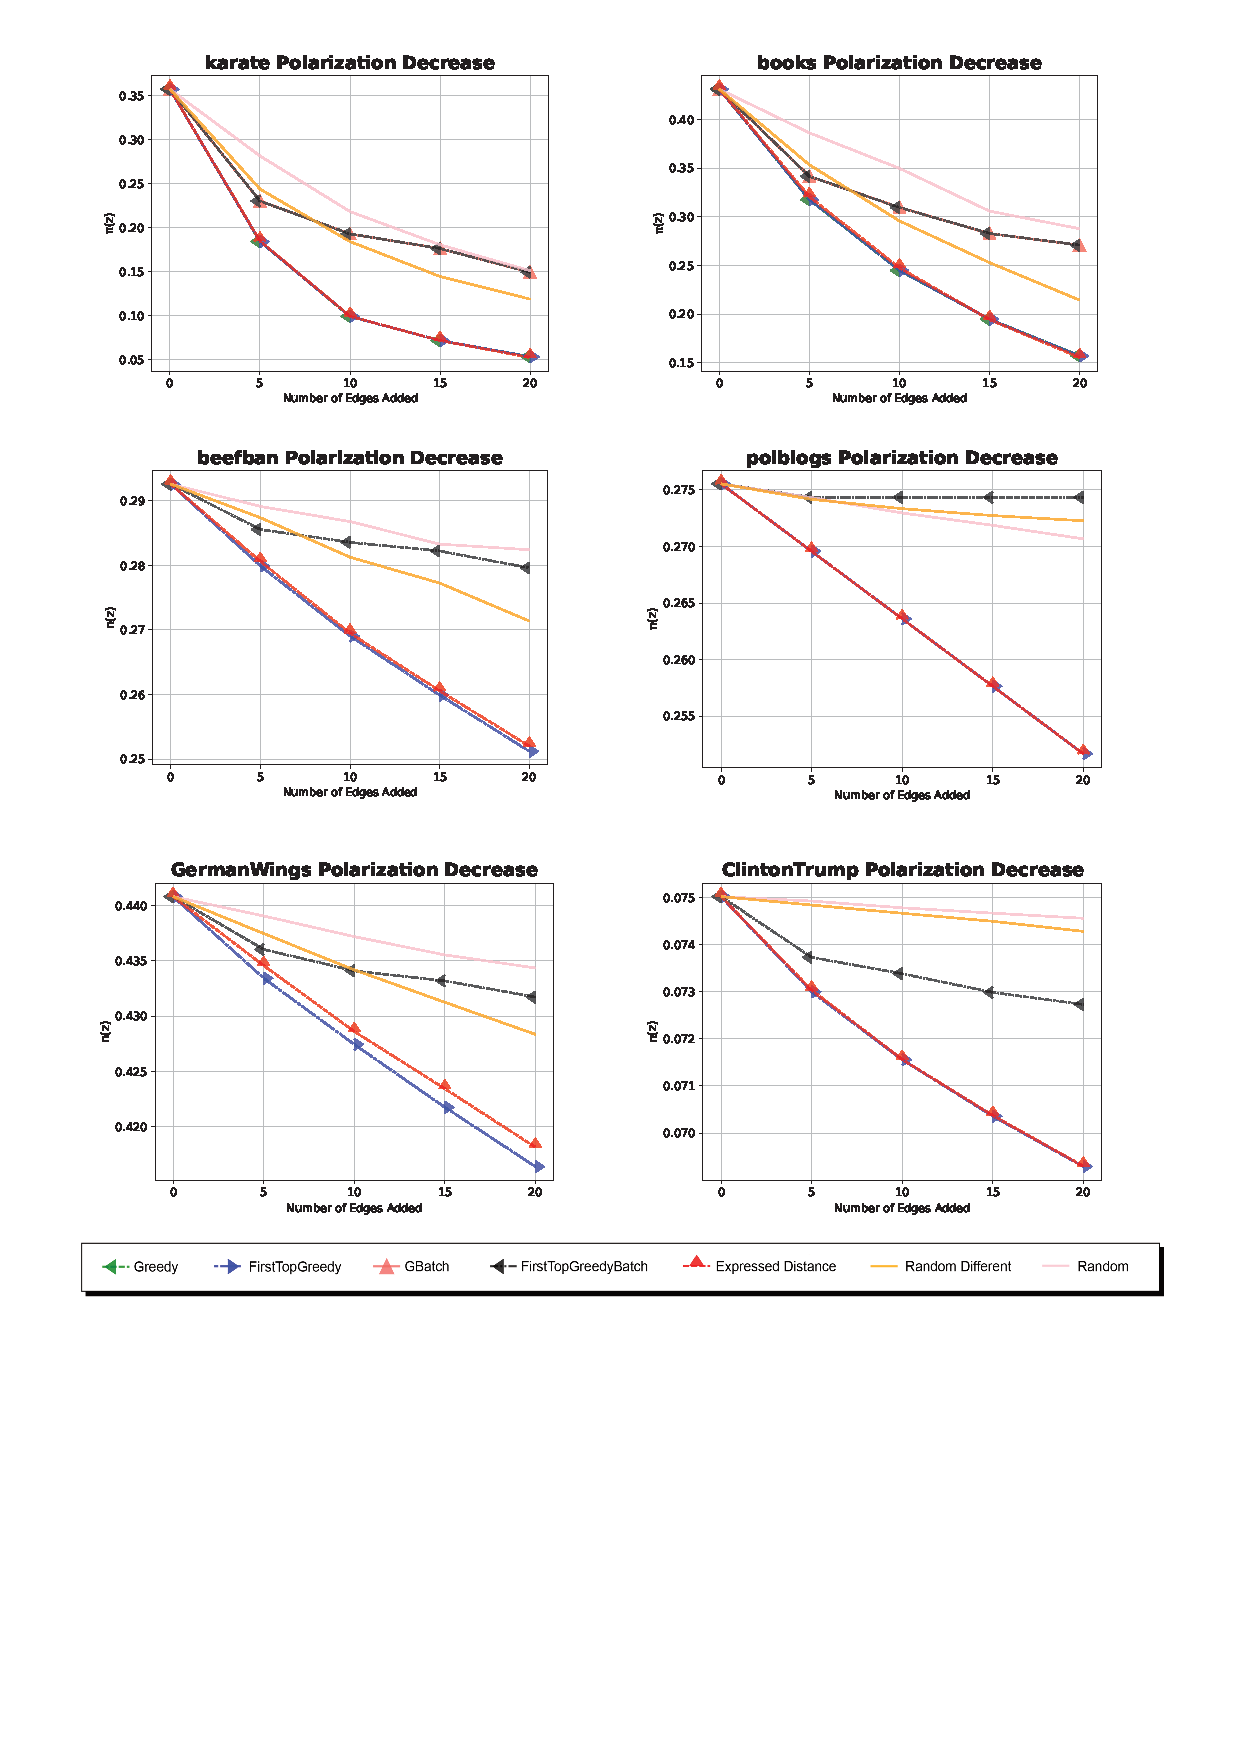
\includegraphics[width=1.2\textwidth]{Figures/heuristics}
	\caption{Comparison of the heuristics between datasets}
	\end{center}
	\label{heuristics_small}
\end{figure}
\clearpage

\noindent We start by applying the heuristics described at~\ref{sec:algorithms} in these 6 datasets. The algorithms perform as expected. The greedy ones have better results but are expensive in time.We can not run the $Greedy$ algorithms in larger datasets due to time limitations.

\begin{itemize}
  \item The Expressed Opinion heuristic that is based on the distance of the opinions performs very well and close to $Greedy$ and are cheap on time.
  \item Batch algorithms perform very poorly, even worse than Random. When adding a new edge the Batch algorithms do not recompute the $Z$ vector. In later edge selections they have a false view of the opinions of the network. For example in a batch version of the $ExpressedOpinion$ the nodes that have the most extreme opinions of each side may reused even if their value is changed after an addition and are no longer the ones with the most extreme values.
 \end{itemize}
 
 \section{A Visualisation of Edge Additions}
\label{sec:vis}
In figure ~\ref{fig:top-10-karate} we can see the 10 edges proposed by the $Greedy$ algorithm. Yellow nodes represent expressed opinions $\epsilon [-1,0)$, green nodes represent expressed opinions $\epsilon (0,1]$ and size shows how central a node is. The green edges are the additions proposed by the algorithm.
\\

\begin{figure}[!htbp]
	\centering
	\captionsetup{justification=centering,margin=2cm}
	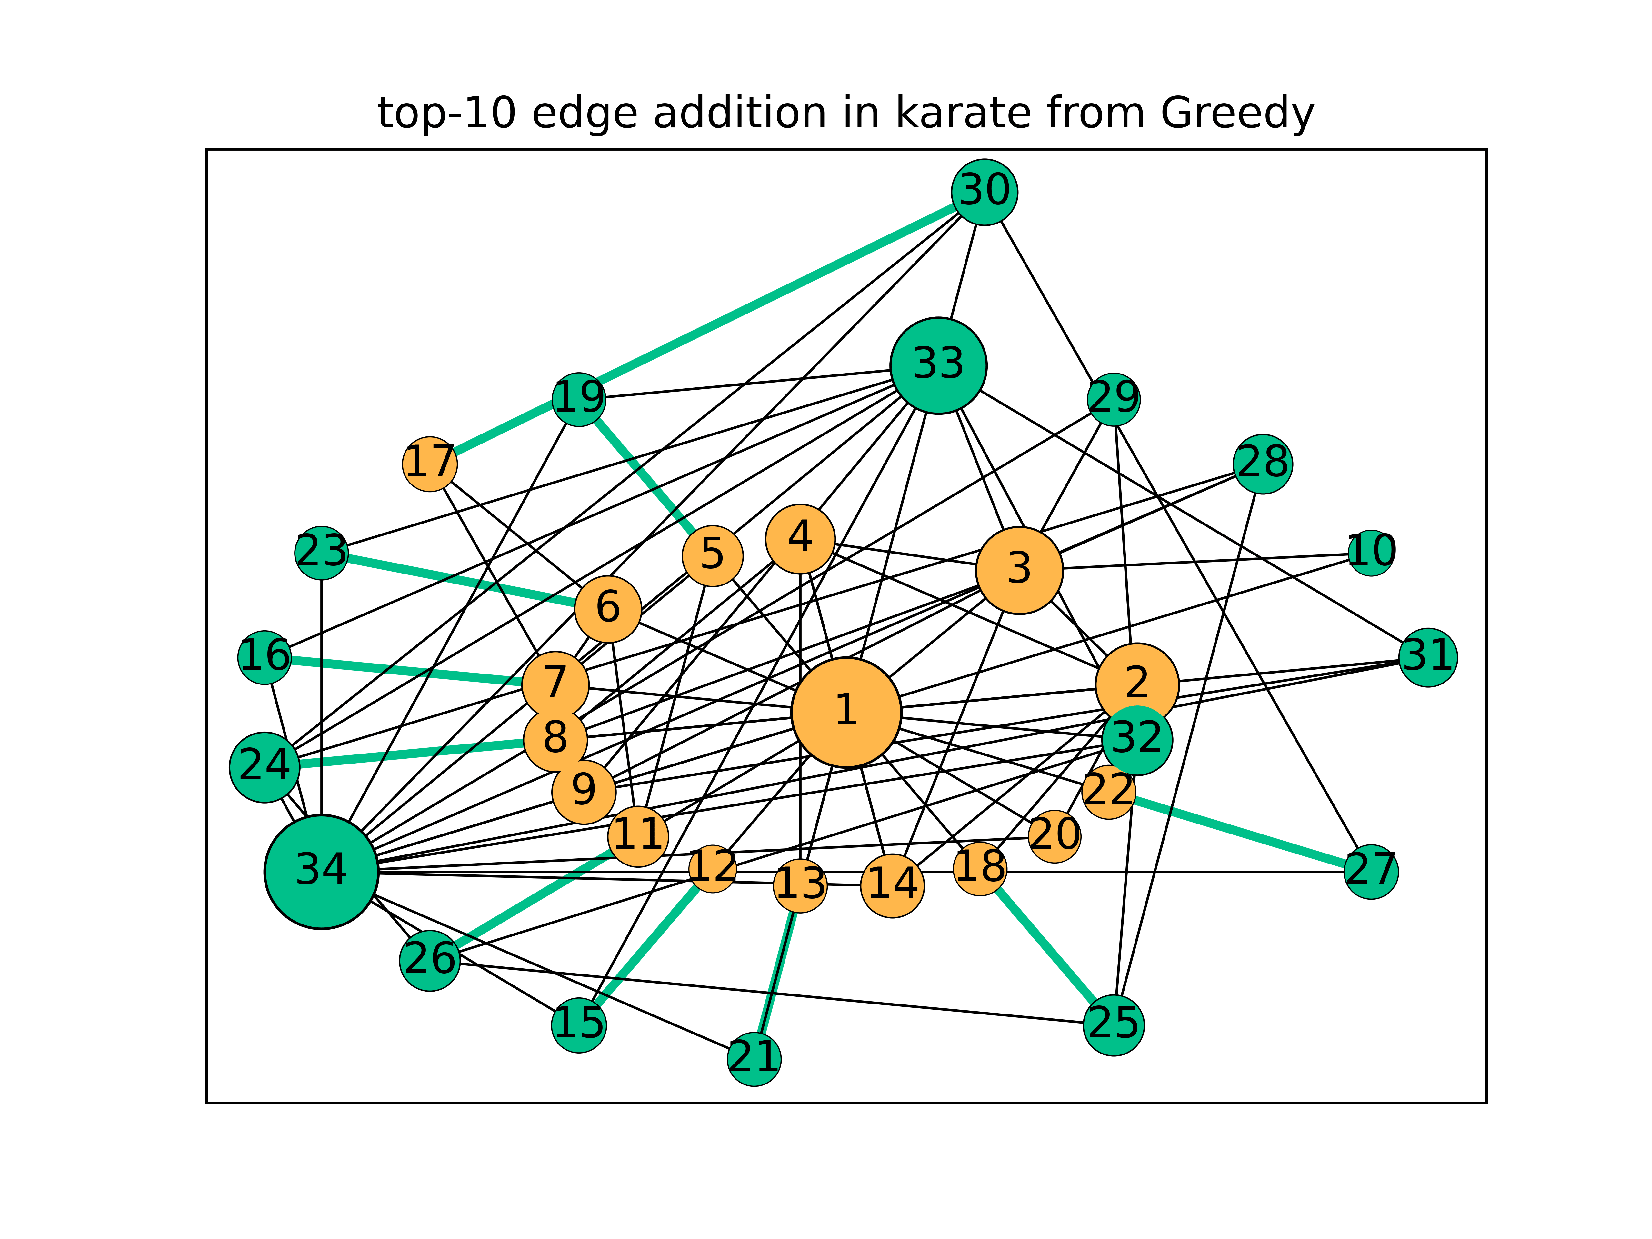
\includegraphics[width=0.65\textwidth]{Figures/top-10_karate_greedy}
	\caption{the top-10 edges proposed by the greedy algorithm}
	\label{fig:top-10-karate}
\end{figure}

